\documentclass{article}

\usepackage[final]{nips_2017}

\usepackage[utf8]{inputenc} % allow utf-8 input
\usepackage[T1]{fontenc}    % use 8-bit T1 fonts
\usepackage{hyperref}       % hyperlinks
\usepackage{url}            % simple URL typesetting
\usepackage{booktabs}       % professional-quality tables
\usepackage{amsfonts}       % blackboard math symbols
\usepackage{nicefrac}       % compact symbols for 1/2, etc.
\usepackage{microtype}      % microtypography
\usepackage{graphicx}

\title{Pun Classification and Location}

% The \author macro works with any number of authors. There are two
% commands used to separate the names and addresses of multiple
% authors: \And and \AND.
%
% Using \And between authors leaves it to LaTeX to determine where to
% break the lines. Using \AND forces a line break at that point. So,
% if LaTeX puts 3 of 4 authors names on the first line, and the last
% on the second line, try using \AND instead of \And before the third
% author name.

\author{
	Shantanu Karnwal
	\texttt{shantanu.karnwal@colorado.edu} \\
	\And
	Amir Kashipazha
	\texttt{amirhossein.kashipazha@colorado.edu} \\
	\And
	Brandon Boylan-Peck
	\texttt{brbo9266@colorado.edu} \\
	\And
	Cathlyn Stone\\
	\texttt{cathlyn.stone@colorado.edu} \\
	\And
	Kenneth Hunter Wapman\\
	\texttt{kennethwapman@colorado.edu} \\
}

\begin{document}

\maketitle

\begin{abstract}
	Pun identification and location are challenging natural language processing 
	tasks. We implemented several algorithms for both, with results which 
	were competitive with the systems presented in the SemEval conference, where
	those tasks were originally defined.
\end{abstract}

%%%%%%%%%%%%%%%%%%%%%%%%%%%%%%%%%%%%%%%%%%%%%%%%%%%%%%%%%%%%%%%%%%%%%%%%%%%%%%%
% Problem Description
%%%%%%%%%%%%%%%%%%%%%%%%%%%%%%%%%%%%%%%%%%%%%%%%%%%%%%%%%%%%%%%%%%%%%%%%%%%%%%%

\section{Overview}

A pun is a form of wordplay within the class of textual phenomena involving
ambiguity where multiple meanings of a word or set of words are played upon to
create a rhetorical effect. They can found in nearly every domain: in
advertising, puns are used to connect a product with a desirable quality; in
literature, puns are used to add a level of meaning and implicaiton; in
conversation, puns add humor to the topic at hand.

Understanding a pun often requires the integration of information from a large
number of contexts; syntax, semantics, and pragmatics all frequently come into
play. 

\subsection{Motivation}

It would be desirable for machines to be able to identify, comprend, and
generate puns for many reasons. A pun generator could facilitate slogan
generation, which would be useful in advertising and dialogue agents; a pun
identify could be used to improve machine translations, where literal
translation of puns rarely conveys the original text's message; a pun
comprehension system would be helpful for large-scale textual analyses of the
kind increasingly being employed in the digital humanities.

A heterographic pun involves a word which sounds similar to another word which
is spelled slightly differently.

We worked on two tasks related to puns: detection location.

\subsection{Pun Structure}

There are many types of puns.

In our work, we focused on two types: homographic puns and heterographic puns. 
\begin{itemize}
	\item {\textbf{Homographic}: A pun involving two words whose spellings are
		the same but have different meanings.\\ \textit{I used to be a banker
		but I lost \textbf{interest}.}}
	\item {\textbf{Heterographic}: A pun involves two or more words which sound
		alike but are spelled differently.\\ \textit{Two construction workers
		had a \textbf{stairing} contest.}}
\end{itemize}

\begin{itemize}

\item homographic: 
A homographic pun involves two words which are spelled the same but have
different meanings.

\item heterographic
\item other types

\end{itemize}

\begin{center}

	homographic pun example
  % \url{https://cmt.research.microsoft.com/NIPS2017/}
\end{center}

\begin{center}
	heterographic pun example
  % \url{https://cmt.research.microsoft.com/NIPS2017/}
\end{center}


\subsection{Dataset}

We trained and tested our algorithms on the test sets used to appraise the
competing systems in SemEval2017 Task 7. The dataset for each of the tasks we
worked on was split into two parts: homographic and heterographic. We modified
the characteristics of these datasets to address some issues we found. Namely,
the original datasets for the detection tasks for both heterographic and
homographic puns had a pun/non-pun split of 70/30. The non-pun sentences for
each type of pun were, however, non-overlapping, so we simply modified each pun
type's dataset to include \emph{all} non-puns from either dataset, giving us a
more even ratio of pun/non-pun.

\subsection{Tasks}

here we will talk about the problems we worked on.

Pun detection is a binary classification problem: given a sequence of words (a
sentence), determine whether or not that sentence contains a pun. Given the
binary nature of the solution space and the highly non-linear input space,
machine learning seems a natural choice.

Pun location is less straightforward: given a set of words known to contain a
pun, identify the pun word. Though this problem is less amenable to traditional
machine learning algorithms, it can be rephrased to be more similar to one: for
each word in the sentence, determine the likelihood that that word is a pun
given the rest of the sentence. Then, output the word which is most likely to
be a pun based on the output of the previous search.

section references \ref{pun_detection}, \ref{pun_location}, and
\ref{conclusion} below.

%%%%%%%%%%%%%%%%%%%%%%%%%%%%%%%%%%%%%%%%%%%%%%%%%%%%%%%%%%%%%%%%%%%%%%%%%%%%%%%
% Pun Detection
%%%%%%%%%%%%%%%%%%%%%%%%%%%%%%%%%%%%%%%%%%%%%%%%%%%%%%%%%%%%%%%%%%%%%%%%%%%%%%%

\section{Pun Detection}
\label{pun_detection}

here we will talk about pun detection and our algorithms.

\begin{block}{Pun Detection Algorithms}
	{\large 
		\begin{itemize}
			\item {\textbf{Multinomial Naive Bayes}\\
				Our baseline---an easy to implement algorithm which we measured approaches against
			}
			\item {\textbf{Bidirectional LSTM}\\
				An LSTM will form connections between the start and end of a sentence and can handle variable-length sentences.
			}
			\item {\textbf{Linear SVM}\\ 
				Allows us to include an arbitrary set of features.
			}
		\end{itemize}
	}
\end{block}
\subsection{Baseline}

\subsection{Algorithms}

\subsection{Feature Comparison}
We introduced various features to improve accuracy. Table (number ?) shows the them and their indexes. These indexes are represent their related feature in feature related figures. Features were added to the code one by one to find how they improved accuracy. Accuracy change behave differently against each feature. For example, accuracy did not increased or decreased with positive and negative. In the other hand, unigram hiked up accuracy to 100 percent which means over fitting. We eliminated features which did effect accuracy from our code. Finally, we ended up using 11 features, index 0 to 10, for feature comparison.\\

In order to find what combinations of feature makes the largest accuracy, we used combination rule to find all possible combination of our 11 features. This made 2047 feature combination. We run code for each combination separately for homographic and heterographic pun, 4089 for both of them. Figures (add figure numbers here) shows the 10 largest accuracy of testing and training set for homographic and heterographic.\\



\begin{center}
\begin{tabular}{l l} 
\toprule
\textbf{Index} 	&	\textbf{Feaute Name}	\\
\midrule
0	&	Lesk Algorithm	\\
1	&	Pos	\\
2	&	tfidf	\\
3	&	Embeddings	\\
4	&	Unigram	\\
5	&	Number of Homophone in Pun	\\
6	&	Number of Each Homophone in Pun	\\
7	&	Homophone is in Pun or Not	\\
8	&	Idiom is in Pun or Not	\\
9	&	Antonyms is in Pun or Not	\\
10	&	Homonym is in Pun or Not	\\
11	&	Bigram	\\
12	&	Trigram	\\
13	&	Positives	\\
14	&	Negatives	\\
15	&	All or First Caps	\\
\bottomrule
\end{tabular}
\end{center}



\begin{figure}
  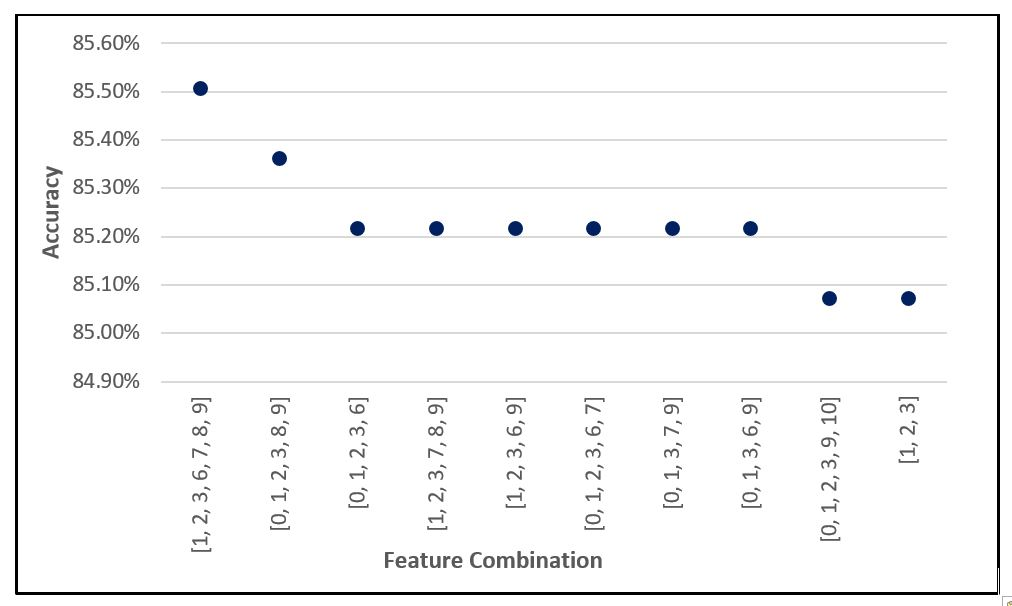
\includegraphics{figures/Accuracy_on_Test_Set_for_Homographic_Pun.JPG}
  \caption{Figure NUMBER ? - Accuracy on Test Set for Homographic Pun}
  \label{fig:boat1}
\end{figure}




%%%%%%%%%%%%%%%%%%%%%%%%%%%%%%%%%%%%%%%%%%%%%%%%%%%%%%%%%%%%%%%%%%%%%%%%%%%%%%%
% Pun Location
%%%%%%%%%%%%%%%%%%%%%%%%%%%%%%%%%%%%%%%%%%%%%%%%%%%%%%%%%%%%%%%%%%%%%%%%%%%%%%%
\section{Pun Location}
\label{pun_location}

\subsection{Baseline}

\subsection{Algorithms}

\section{Results}
\label{results}

\subsection{Pun Detection}
Here's how we think we did.
\subsubsection{Evaluation}
\subsubsection{Results}
here are our results. here's the baseline. here's semeval's

\subsubsection{Error Analysis}

\subsection{Pun Location}
Here's how we think we did.
\subsubsection{Evaluation}
f score etc etc
\subsubsection{Results}
here are our results. here's the baseline. here's semeval's
\subsubsection{Error Analysis}

%%%%%%%%%%%%%%%%%%%%%%%%%%%%%%%%%%%%%%%%%%%%%%%%%%%%%%%%%%%%%%%%%%%%%%%%%%%%%%%
% Conclusion
%%%%%%%%%%%%%%%%%%%%%%%%%%%%%%%%%%%%%%%%%%%%%%%%%%%%%%%%%%%%%%%%%%%%%%%%%%%%%%%

\section{Conclusion}
\label{conclusion}

\subsection{Who Did What}

\begin{itemize}

\item Shantanu Karnwal worked on:
	\begin{itemize}
		\item poster layout
	\end{itemize}
\item Amir Kashipazha
	\begin{itemize}
		\item features (antonyms, idioms, sentiment)
		\item the feature comparison for the SVM used for SGD Pun Detection
	\end{itemize}
\item Brandon Boylan-Peck
	\begin{itemize}
		\item poster bar graphs
	\end{itemize}
\item Cathlyn Stone
	\begin{itemize}
		\item the interactive web app
		\item the framework for running classifiers
		\item features (lesk algorithm, POS)
		\item the SVM used in the SGD Pun Detection algorithm
		\item the sliding window MEMM used in Pun Location
		\item the ensemble algorithm
		\item algorithm cross validation
		\item the Bidirectional LSTM used for Pun Location
		\item evaluation of the Pun Detection algorithms
		\item the model caching architecture
	\end{itemize}
\item Kenneth Hunter Wapman
	\begin{itemize}
		\item data loading and manipulation
		\item the baseline algorithm for Pun Detection
		\item features (word embeddings)
		\item the framework for running classifiers
		\item the sliding window MEMM used in Pun Location
		\item the Bidirectional LSTM used for Pun Location
		\item the Bidirectional LSTM used for Pun Detection
		\item evaluation of the Pun Location algorithms
		\item poster content
		\item report content
	\end{itemize}
\end{itemize}

\subsection{What Went Well}

\subsection{What We Could Have Done Better}

\subsection{Future Work}

An obvious shortcoming of our system is that it will only predict \emph{one
word} as the pun word, but, and the idea that there is \emph{one word} the makes
a pun is somewhat dubious (not to mention that compound puns exist). Consider
the following pun: 
\begin{center}
	\emph{The rabbi got hit on the temple.}
\end{center}
Our system would say that the punword is ``temple'', but that is really only half
the story; if the word ``rabbi'' were replaced with, say, ``monk'', there would
be no pun. The ability to identify the words \emph{involved} in a pun would be
much more useful, and to the authors of this report, more interesting.

Of obvious interest is the ability to detect further types of puns, perhaps
using context provided by differt types of data; it would be extremely
interesting to create a system which could identify visual puns. 

It would be of interest to say \emph{what} about the words in a sentence make it
a pun. In other words, the creation of a system which could interpret puns.

A more out-there hope would be a system which could generate puns, perhaps being
given a sentence and a pair of word senses.

\subsubsection*{Acknowledgments}

here's where we acknowledge stuff

%%%%%%%%%%%%%%%%%%%%%%%%%%%%%%%%%%%%%%%%%%%%%%%%%%%%%%%%%%%%%%%%%%%%%%%%%%%%%%%
% References
%%%%%%%%%%%%%%%%%%%%%%%%%%%%%%%%%%%%%%%%%%%%%%%%%%%%%%%%%%%%%%%%%%%%%%%%%%%%%%%
\section*{References}

\medskip

\small

[1] Oele, D., \& Evang, K.\ (2017) BuzzSaw at SemEval-2017 Task 7:
Global vs. Local Context for Interpreting and Locating Homographic English Puns
with Sense Embeddings. Proceedings of the 11th International Workshop on
Semantic Evaluations (SemEval-2017), pages 444–448, Vancouver, Canada, August 3
- 4, 2017. 2017 © Association for Computational Linguistics.

[2] Pedersen, T.\ (2017) Duluth at SemEval-2017 Task 7: Puns Upon a Midnight
Dreary, Lexical Semantics for the Weak and Weary. Proceedings of the 11th
International Workshop on Semantic Evaluations (SemEval-2017), pages 416–420,
Vancouver, Canada, August 3 - 4, 2017. 2017 © Association for Computational
Linguistics.

[3] Xiu, Y., Lan, M., \& Wu, Y.\ (2017). ECNU at SemEval-2017 Task 7: Using
Supervised and Unsupervised Methods to Detect and Locate English Puns.
Proceedings of the 11th International Workshop on Semantic Evaluations
(SemEval-2017), pages 453–456, Vancouver, Canada, August 3 - 4, 2017. 2017 ©
Association for Computational Linguistics.

[4] Hurtado, L., Segarra, E., Pla, F., Carrasco, P., \& Gonzalez, J.A..
(2017). ELiRF-UPV at SemEval-2017 Task 7: Pun Detection and Interpretation.
Proceedings of the 11th International Workshop on Semantic Evaluations
(SemEval-2017), pages 440–443, Vancouver, Canada, August 3 - 4,
2017. 2017 © Association for Computational Linguistics.

[5] Indurthi, V., \&  Reddy, O.S.\ (2017). Fermi at SemEval-2017 Task
7: Detection and Interpretation of Homographic puns in English Language.
Proceedings of the 11th International Workshop on Semantic Evaluations
(SemEval-2017), pages 457–460, Vancouver, Canada, August 3 - 4, 2017. 2017 ©
Association for Computational Linguistics.

[6] Samuel Doogan, Aniruddha Ghosh, Hanyang Chen, and Tony Veale. 2017. Idiom
Savant at Semeval-2017 Task 7: Detection and Interpretation of English Puns.
Proceedings of the 11th International Workshop on Semantic Evaluations
(SemEval-2017), pages 103–108, Vancouver, Canada, August 3 - 4, 2017. 2017 ©
Association for Computational Linguistics.

[7] Das, D. \& Pramanick, A. (2017). JU\_CSE\_NLP at SemEval 2017 Task 7:
Employing Rules to Detect and Interpret English Puns. Proceedings of the 11th
International Workshop on Semantic Evaluations (SemEval-2017), pages 432–435,
Vancouver, Canada, August 3 - 4, 2017. 2017 © Association for Computational
Linguistics.

[8] Mikhalkova, E. \& Karyakin, Y. (2017). PunFields at SemEval-2017 Task 7:
Employing Roget’s Thesaurus in Automatic Pun Recognition and Interpretation.
Proceedings of the 11th International Workshop on Semantic Evaluations
(SemEval-2017), pages 426–431, Vancouver, Canada, August 3 - 4, 2017. 2017 ©
Association for Computational Linguistics.

[9] Bahuleyan, H. \& Vechtomova, O. (2017). UWaterloo at SemEval-2017 Task 8:
Detecting Stance towards Rumours with Topic Independent Features. Proceedings
of the 11th International Workshop on Semantic Evaluations (SemEval-2017),
pages 461–464, Vancouver, Canada, August 3 - 4, 2017. 2017 © Association for
Computational Linguistics.

[10] Vadehra, A. (2017). UWAV at SemEval-2017 Task 7: Automated feature-based
system for locating puns. Proceedings of the 11th International Workshop on
Semantic Evaluations (SemEval-2017), pages 449–452, Vancouver, Canada, August 3
- 4, 2017. 2017 © Association for Computational Linguistics.

[11] Sevgili, O., Ghotbi, N., \& Tekir, S. (2017). N-Hance at SemEval-2017 Task
7: A Computational Approach using Word Association for Puns. Proceedings of the
11th International Workshop on Semantic Evaluations (SemEval-2017), pages
436–439, Vancouver, Canada, August 3 - 4, 2017. 2017 © Association for
Computational Linguistics.

%%%%%%%%%%%%%%%%%%%%%%%%%%%%%%%%%%%%%%%%%%%%%%%%%%%%%%%%%%%%%%%%%%%%%%%%%%%%%%%
% Misc Style examples
%%%%%%%%%%%%%%%%%%%%%%%%%%%%%%%%%%%%%%%%%%%%%%%%%%%%%%%%%%%%%%%%%%%%%%%%%%%%%%%
\section{Style Stuff}
\verb+this is code-ish looking+ 

here's a percent: $\sim$$15\%$
\textbf{boldboldbold}
\emph{italics}

here's a fraction: \nicefrac{1}{4}

\paragraph{}This is paragraphed
\begin{verbatim}
   \citet{hasselmo} investigated\dots
\end{verbatim}
produces
\begin{quote}
  Hasselmo, et al.\ (1995) investigated\dots
\end{quote}

ref number:\ [4]

footnotes.\footnote{they go after the period}

\begin{figure}[h]
  \centering
  \fbox{\rule[-.5cm]{0cm}{4cm} \rule[-.5cm]{4cm}{0cm}}
  \caption{Sample figure caption.}
\end{figure}

Table~\ref{sample-table}.

use \verb+booktabs+ package for tables
\begin{center}
  \url{https://www.ctan.org/pkg/booktabs}
\end{center}

\begin{table}[t]
  \caption{Sample table title}
  \label{sample-table}
  \centering
  \begin{tabular}{lll}
    \toprule
    \multicolumn{2}{c}{Part}                   \\
    \cmidrule{1-2}
    Name     & Description     & Size ($\mu$m) \\
    \midrule
    Dendrite & Input terminal  & $\sim$100     \\
    Axon     & Output terminal & $\sim$10      \\
    Soma     & Cell body       & up to $10^6$  \\
    \bottomrule
  \end{tabular}
\end{table}

\end{document}
